\documentclass[xelatex,14pt]{beamer}
\usetheme{metropolis}
%\usefonttheme{professionalfonts} % using non standard fonts for beamer
\usefonttheme{serif}
\usepackage{helvet}
\usepackage[english]{babel}
\usepackage{graphicx}
\usepackage{textpos}
\usepackage{xcolor}
\definecolor{mauve}{rgb}{0.86, 0.82, 1.0}
\definecolor{dkgreen}{rgb}{0,0.6,0}
\usepackage{pgfpages}
\usepackage{listings}

\lstdefinelanguage{d}{
	morekeywords={abstract,alias,align,asm,assert,auto,body,bool,break,byte,
		case,cast,catch,cdouble,cent,cfloat,char,class,const,continue,creal,
		dchar,debug,default,delegate,delete,deprecated,do,double,else,enum,
		export,extern,false,final,finally,float,for,foreach,foreach_reverse,
		function,goto,idouble,if,ifloat,immutable,import,in,inout,int,
		interface,invariant,ireal,is,lazy,long,macro,mixin,module,new,nothrow,
		null,out,override,package,pragma,private,protected,public,pure,real,
		ref,return,scope,shared,short,static,struct,string,wstring,dstring,
		super,switch,synchronized,template,this,throw,true,try,typedef,typeid,
		typeof,ubyte,ucent,uint,ulong,union,unittest,ushort,version,void,
		volatile,wchar,while,with,size_t,hash_t,__traits
	},
	sensitive=True,
	morecomment=[l]{//},
	morecomment=[s]{/\*}{\*/},
	morestring=[b]"
}
\lstdefinelanguage{typescript}{
	morekeywords={abstract,alias,align,asm,assert,auto,body,bool,break,byte,
		case,cast,catch,cdouble,cent,cfloat,char,class,const,continue,creal,
		dchar,debug,default,delegate,delete,deprecated,do,double,else,enum,
		export,extern,false,final,finally,float,for,foreach,foreach_reverse,
		function,goto,idouble,if,ifloat,immutable,import,in,inout,int,
		interface,invariant,ireal,is,lazy,long,macro,mixin,module,new,nothrow,
		null,out,override,package,pragma,private,protected,public,pure,real,
		ref,return,scope,shared,short,static,struct,string,wstring,dstring,
		super,switch,synchronized,template,this,throw,true,try,typedef,typeid,
		typeof,ubyte,ucent,uint,ulong,union,unittest,ushort,version,void,
		volatile,wchar,while,with,size_t,hash_t,number,extends,constructor
	},
	sensitive=True,
	morecomment=[l]{//},
	morecomment=[s]{/\*}{\*/},
	morestring=[b]",
	morestring=[b]'
}


\lstset{
	language=d,
	basicstyle=\footnotesize\ttfamily, % Standardschrift
	numbers=left,               % Ort der Zeilennummern
	numberstyle=\tiny,          % Stil der Zeilennummern
	%stepnumber=2,               % Abstand zwischen den Zeilennummern
	captionpos=b,
	numbersep=5pt,              % Abstand der Nummern zum Text
	tabsize=4,                  % Groesse von Tabs
	extendedchars=true,         %
	breaklines=true,            % Zeilen werden Umgebrochen
	showspaces=false,           % Leerzeichen anzeigen ?
	showtabs=false,             % Tabs anzeigen ?
	%frame=b,
	rulecolor=\color[cmyk]{0.0, 0.0, 0.0, 0.316},
	xleftmargin=17pt,
	%xleftmargin=0pt,
	framexleftmargin=17pt,
	framexrightmargin=5pt,
	framexbottommargin=4pt,
	keywordstyle=\color{blue},          % keyword style
	commentstyle=\color{dkgreen},       % comment style
	stringstyle=\color{red},         % string literal style
	showstringspaces=false,    % Leerzeichen in Strings anzeigen ?        
	escapeinside={/+}{+/},
	title=\lstname,
    postbreak=\raisebox{0ex}[0ex][0ex]{\ensuremath{\color{red}\hookrightarrow\space}}
}

%\setbeamertemplate{note page}{\pagecolor{yellow!5}\insertnote}\usepackage{palatino}
%\setbeameroption{show notes on second screen}

\beamertemplatenavigationsymbolsempty

\usepackage{xkeyval}
%\presetkeys{todonotes}{inline}{}
\usepackage[disable]{todonotes}

\title{Asynchronous Single Page Applications without a Line of HTML or
Javascript.}
\subtitle{Or why D is just awesome}
\author{Robert "burner" Schadek}
\date{May 5, 2016}
\institute{DConf}

\begin{document}
\maketitle

\begin{frame}
	\frametitle{Javascript and HTML are \textbf{awesome}}
	\begin{itemize}
		\item No explicit types
		\item Variables may be undefined
		\item Repetition repetition repetition
		\item No templates
		\item No compile time function execution
		\item No compile time
	\end{itemize}
	\note[item]{Very quickly go through the points and stop for dramatic pause}
\end{frame}


\begin{frame}[plain]
\begin{textblock*}{0cm}(-1cm,-4.2cm)
	
\includegraphics[width=1.0\paperwidth]{picardriker.jpg}
\end{textblock*}
	\note[item]{I know what you are thinking.}
	\note[item]{Walter, Andrei and the other screwed up letting me present
	here.}
\end{frame}

\begin{frame}
	\frametitle{Goals}	
	\begin{itemize}
		\item Retain type-information of data from DB to Client's Browser
			\pause
		\item Keeping things DRY	
			\pause
		\item Performance
			\pause
		\item Get things done
	\end{itemize}
\end{frame}

\section{Vibe.d and Diet}
\begin{frame}
	\frametitle{Vibe.d}
	\begin{itemize}
		\item Powerful asynchronous I/O and web toolkit for D
		\item Uses Fibers and Threads
			\pause
			\begin{itemize}
				\item \(n \rightarrow m\) mapping
				\item \lstinline@yield()@
				\item async IO
			\end{itemize}
			\pause
		\item async DB connectivity for MongoDB, Redis, MySQL
		\item You don't need to care about async
		\item Web interface generator
		\item REST interface generator
	\end{itemize}
\end{frame}

\subsection{Vibe.d}
\begin{frame}
	\frametitle{REST Interface Generator}
	\lstinputlisting[basicstyle=\footnotesize,caption={},linerange=5-9,
		firstnumber=5,numbers=none,xleftmargin=-0.7cm
	]{Sources/VibeAngularExample/source/app.d}
	\pause
	\lstinputlisting[basicstyle=\footnotesize,caption={},linerange=10-19,
		firstnumber=5,numbers=none,xleftmargin=-0.7cm
	]{Sources/VibeAngularExample/source/app.d}
\end{frame}
\begin{frame}
	\frametitle{REST Interface Generator}
	\lstinputlisting[basicstyle=\footnotesize,caption={},linerange=30-34,
		firstnumber=30,numbers=none,xleftmargin=-1.5cm
	]{Sources/VibeAngularExample/source/app.d}
	\pause
	\vspace{1cm}
	\lstinputlisting[basicstyle=\footnotesize,caption={},linerange=1-4,
		firstnumber=1,xleftmargin=-0.7cm,numbers=none
	]{Sources/VibeAngularExample/source/weather.d}
\end{frame}

\subsection{Angular Typescript}
\begin{frame}
	\frametitle{AngularJS Typescript}
	\lstinputlisting[language=typescript,basicstyle=\footnotesize,caption={},
		linerange=16-20, firstnumber=16,numbers=none,xleftmargin=-0.7cm
	]{Sources/VibeAngularExample/public/myapp.ts}
	\pause
	\lstinputlisting[language=typescript,basicstyle=\footnotesize,caption={},
		linerange=21-24, firstnumber=16,numbers=none,xleftmargin=-0.7cm
	]{Sources/VibeAngularExample/public/myapp.ts}
	\pause
	\lstinputlisting[language=typescript,basicstyle=\footnotesize,caption={},
		linerange=25-32, firstnumber=16,numbers=none,xleftmargin=-0.7cm
	]{Sources/VibeAngularExample/public/myapp.ts}
\end{frame}

\begin{frame}
	\frametitle{AngularJS Typescript}
	\lstinputlisting[language=typescript,basicstyle=\footnotesize,caption={},
		linerange=34-39, firstnumber=16,numbers=none,xleftmargin=-1.4cm
	]{Sources/VibeAngularExample/public/myapp.ts}
\end{frame}

\subsection{Diet}
\begin{frame}
	\frametitle{Diet}
	\lstinputlisting[language={},basicstyle=\small,caption={},
		linerange=4-13,
		firstnumber=4,numbers=none,xleftmargin=-0.7cm
	]{Sources/VibeAngularExample/views/index.dt}
	\pause
	\lstinputlisting[language={},basicstyle=\small,caption={},
		linerange=1-3,
		firstnumber=1,numbers=none,xleftmargin=-0.7cm
	]{Sources/VibeAngularExample/views/index.dt}
\end{frame}
\begin{frame}
	\frametitle{Diet}
	\lstinputlisting[language={},basicstyle=\small,caption={},
		linerange=1-20,
		firstnumber=1,numbers=none,xleftmargin=-0.7cm
	]{Sources/VibeAngularExample/views/main.dt}
\end{frame}

\section{Live Demo}

\section{Dataflow from the Server to the Frontend and back again}
\begin{frame}
	\frametitle{Dataflow from the Server to the Frontend and back again}
	\lstinputlisting[basicstyle=\small,title={Dlang},linerange=1-4,
		firstnumber=1,numbers=none
	]{Sources/VibeAngularExample/source/weather.d}
	\pause
	\lstinputlisting[language=typescript,basicstyle=\small,
		title={Typescript}, linerange=16-19, firstnumber=16,numbers=none
	]{Sources/VibeAngularExample/public/myapp2.ts}
\end{frame}

\begin{frame}[fragile]
	\frametitle{dstructtotypescript}
\begin{lstlisting}[numbers=none,language=bash]
dstructtotypescript -i weather.d -p weather.ts -s Weather
\end{lstlisting}
\pause
%dstructtotypescript control flow:
%\begin{enumerate}
%	\item Write D source file containing magic and content of weather.d	
%	\item rdmd source file
%	\item Use typescript file containing \lstinline@struct Weather@ converted
%		to Typescript
%\end{enumerate}
	\vspace{-1cm}
\begin{figure}[h]
	\hspace*{-1cm}
	\begin{tikzpicture}
		\node at (-2.1,4) (D) {
			\lstinputlisting[numbers=none,basicstyle=\footnotesize,caption={},
				linerange=1-4, firstnumber=1
			]{Sources/VibeAngularExample/source/weather.d}
		};
		\pause
		\node at (-0.5,1) (F) {
\begin{lstlisting}[language=d,numbers=none,basicstyle=\footnotesize,caption={}]
import std.format;

foreach(it; __traits(allMembers, Weather))
\end{lstlisting}
		};
		\pause
		\node at(5,3.0) (T) {
			\lstinputlisting[numbers=none,language=typescript,basicstyle=\footnotesize,
				caption={}, linerange=16-19, firstnumber=16
			]{Sources/VibeAngularExample/public/myapp.ts}
		};

	\draw[->,line width=0.2mm,black] (D) -- (T);
	\draw[->,line width=0.2mm,black] (F) -- (T);
	\end{tikzpicture}
	
\end{figure}
\end{frame}

\section{Everything is wrong}
\begin{frame}
\begin{textblock*}{0cm}(-1cm,-4.2cm)
	
\includegraphics[width=1.0\paperwidth]{picarddday.jpg}
\end{textblock*}
\end{frame}


\fontsize{12pt}{7.2}\selectfont

\begin{frame}
	\frametitle{Everything is wrong}
	\begin{itemize}
		\item All we solved was a tiny specific problem
		\item What about server to database
		\item What if we would use Dart instead of Typescript
		\item How do we communicate the overall architecture
		\item How do we keep the architecture in sync with the code
		\item How do we communicate with non-developer
		\item ...
		\pause
		\item {\large How do we deal with change?}
	\end{itemize}
\end{frame}

\begin{frame}
	\frametitle{Everything is still wrong}
	\begin{itemize}
		\onslide<1->{\item Waterfall Model} \onslide<2->{\(\leftarrow\) 
			no change, never}
		\onslide<7->{\item UML} \onslide<8->{\(\leftarrow\) just kill me
			already}

		\item[] { \onslide<1-8>{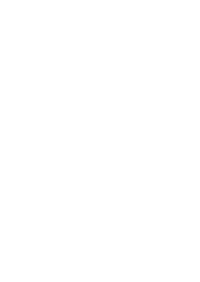
\includegraphics[width=0.3\textwidth]{Stick1.png}}
			\only<9>{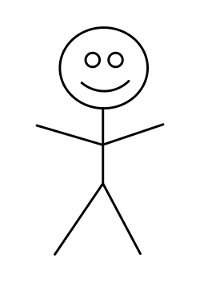
\includegraphics[width=0.3\textwidth]{Stick.png}}
			\only<10>{\hspace{-1.31mm}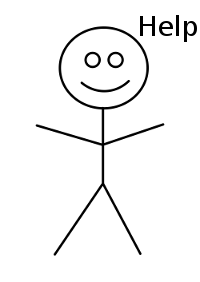
\includegraphics[width=0.3\textwidth]
				{Stick2.png}}
		}

		\onslide<5->{\item Agile Methods} \onslide<6->{\(\leftarrow\) just
			hacking, with fancy names}
		\onslide<3->{\item Hacking} \onslide<4->{\(\leftarrow\) no plan
			to speak of, just change}
		
	\end{itemize}
	
\end{frame}

\begin{frame}
	\frametitle{What do we want}
	\begin{itemize}
		\item Speak about the system at different levels of detail\\
		with different people
		\item Quickly introduce people to the system
		\item Keep data classes (Model) synchronized across
		\begin{itemize}
			\item Frontend
			\item Server
			\item Database
		\end{itemize}
		\item Write only one model for everything, to keep stuff in sync
		\item Have description line based, because git
		\item Generate everything possible from the model
	\end{itemize}
\end{frame}

\section{Introducing the C4 Architecture}
\begin{frame}[plain]
\begin{textblock*}{0cm}(-1cm,-4.7cm)
	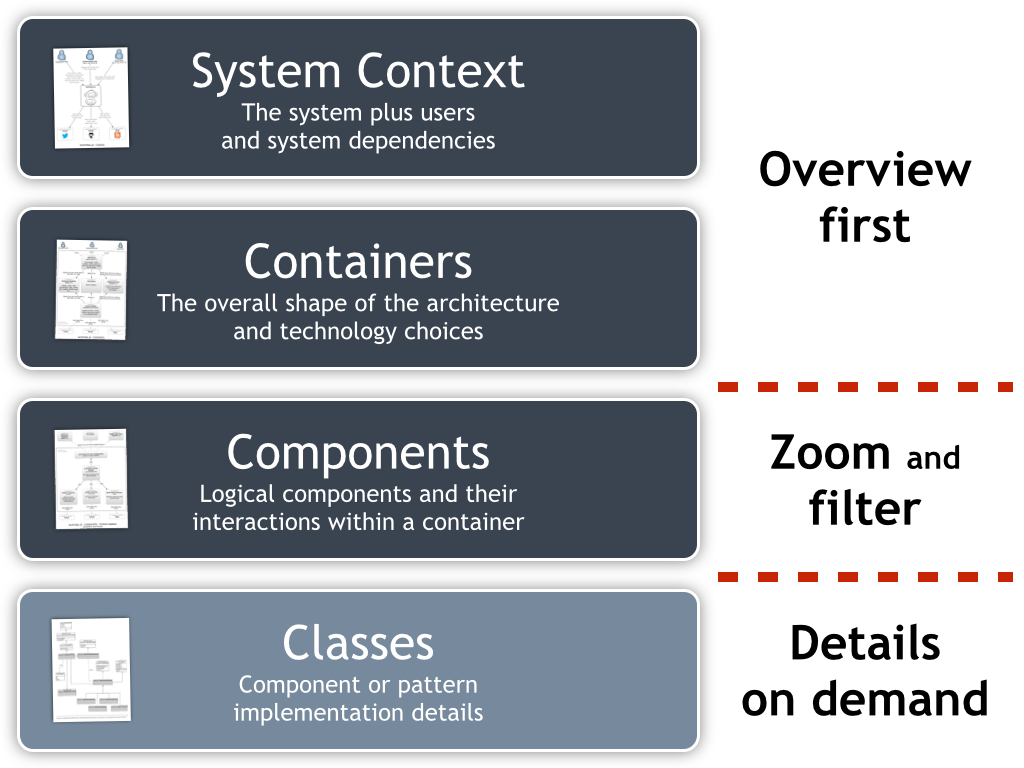
\includegraphics[width=1.0\paperwidth]{c4overview.png}
\end{textblock*}
\end{frame}
\begin{frame}[plain]
\begin{textblock*}{0cm}(-1cm,-4.7cm)
	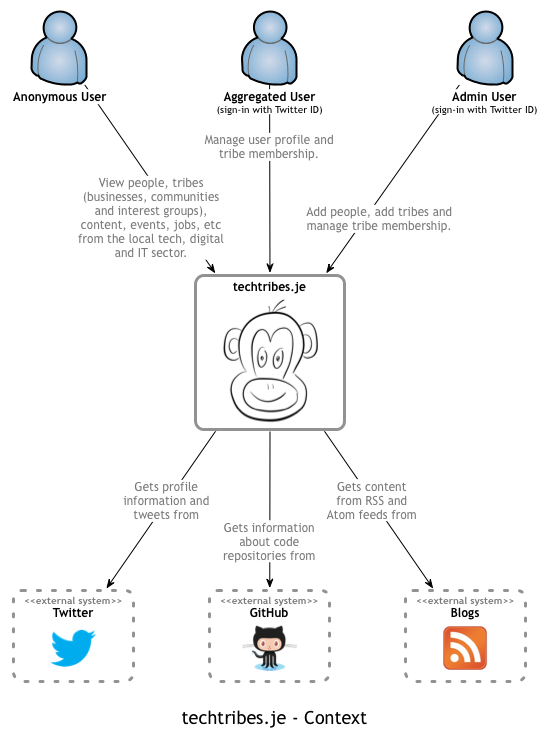
\includegraphics[width=1.0\paperwidth]{c4systemcontext.png}
\end{textblock*}
\end{frame}
\begin{frame}[plain]
\begin{textblock*}{0cm}(-1cm,-11.7cm)
	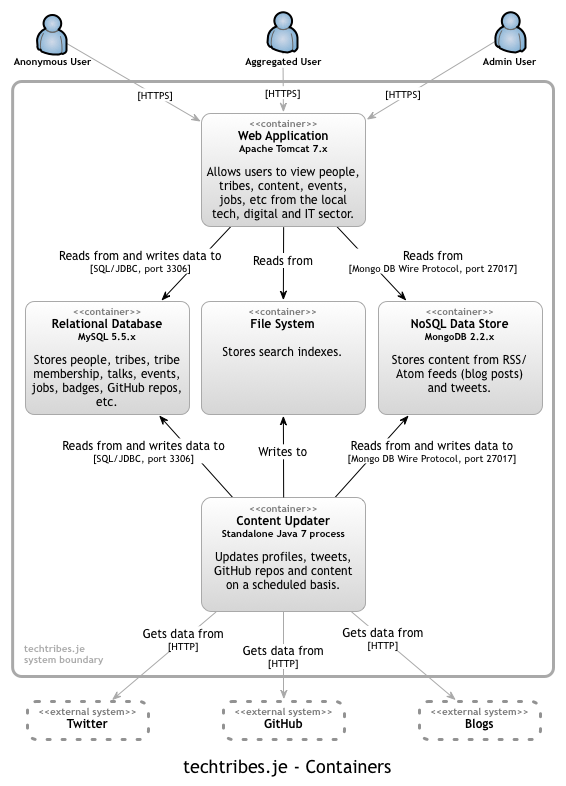
\includegraphics[width=1.0\paperwidth]{c4container.png}
\end{textblock*}
\end{frame}
\begin{frame}[plain]
\begin{textblock*}{0cm}(-1cm,-4.7cm)
	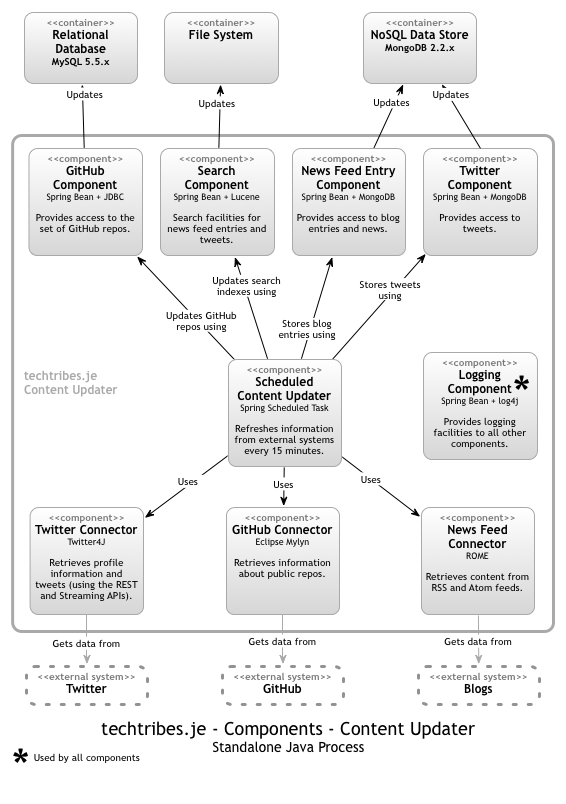
\includegraphics[width=1.0\paperwidth]{c4components.png}
\end{textblock*}
\end{frame}

\begin{frame}
	\frametitle{Structurizr}
	\begin{itemize}
		\item Implements C4 Architecture Model 
		\item Java library to build the model
			\pause
		\begin{itemize}
			\item Its code, its fits into git
		\end{itemize}
			\pause
		\item Structurizr generates code
			\pause
		\item {\huge Only Java and .net}
	\end{itemize}
\end{frame}
\begin{frame}[plain]
\begin{textblock*}{0cm}(-1cm,-4.4cm)
	
\includegraphics[width=1.0\paperwidth]{picardwtf.jpg}
\end{textblock*}
\end{frame}

\section{How hard can it be}
\begin{frame}
	\frametitle{How do we approach the development}
	\begin{itemize}
		\item We're not gonne create a new language\pause, at first\pause,
			most likely
			\pause
		\item The model (ast) is pretty simple
			\pause
		\begin{itemize}
			\item The world
			\item The world has
			\item Actors, software/hardware systems
			\item A software systems has
			\item Containers (everything with a unique pid)
			\item A container has
			\item Components (think \lstinline@module@) and classes
			\item A component has
			\item Components and classes
			\item Classes have members
				\pause
			\item Connections between the above
			\begin{itemize}
				\item UML Association, Aggregation, Composition, Dependency, \(\dots\)
			\end{itemize}
			\item Additional informations, names, descriptions
		\end{itemize}
	\end{itemize}
\end{frame}

\begin{frame}
	\frametitle{Using Degenerator 1/2}
	\lstinputlisting[basicstyle=\footnotesize,caption={},linerange=10-15,
		firstnumber=10,numbers=none,xleftmargin=-1cm
	]{Sources/app.d}
	\pause
	\lstinputlisting[basicstyle=\footnotesize,caption={},linerange=17-19,
		firstnumber=17,numbers=none,xleftmargin=-1cm
	]{Sources/app.d}
\end{frame}
\begin{frame}
	\frametitle{Using Degenerator 2/4}
	\lstinputlisting[basicstyle=\footnotesize,caption={},linerange=45-49,
		firstnumber=45,numbers=none,xleftmargin=-1cm
	]{Sources/app.d}
	\pause
	\lstinputlisting[basicstyle=\footnotesize,caption={},linerange=61-63,
		firstnumber=61,numbers=none,xleftmargin=-1cm
	]{Sources/app.d}
\end{frame}

\begin{frame}
	\frametitle{Using Degenerator 3/4}
	\lstinputlisting[basicstyle=\small,caption={},linerange=61-63,
		firstnumber=61,numbers=none,xleftmargin=-1cm
	]{Sources/app.d}
	\pause
	\lstinputlisting[basicstyle=\small,caption={},linerange=68-71,
		firstnumber=68,numbers=none,xleftmargin=-1cm
	]{Sources/app.d}
\end{frame}
\begin{frame}
	\frametitle{Using Degenerator 4/4}
	\lstinputlisting[basicstyle=\small,caption={},linerange=77-79,
		firstnumber=77,numbers=none,xleftmargin=-1cm
	]{Sources/app.d}
	\pause
	\lstinputlisting[basicstyle=\small,caption={},linerange=90-92,
		firstnumber=90,numbers=none,xleftmargin=-1cm
	]{Sources/app.d}
\end{frame}

\begin{frame}[fragile]
	\frametitle{Types in Degenerator}
	\begin{itemize}
		\item Types \pause e.g. strings are not always strings
		\pause
		\begin{itemize}
			\item D string
			\item MySQL text
			\item C++ std::string
		\end{itemize}
	\end{itemize}
	\pause
	\begin{lstlisting}[basicstyle=\small,xleftmargin=0.2cm,numbers=none]
struct Type {
    string name;
    string[string] typeMapping;
}

auto pwdHash = Type("PasswordString"); /+\pause+/
pwdHash.typeMappings["D"] = "string";
pwdHash.typeMappings["MySQL"] = "VARCHAR(128)";
\end{lstlisting}
	\vspace{-1cm}
%\begin{itemize}
%	\item Similar types with different behaviour across containers
%\end{itemize}
\end{frame}

\begin{frame}
	\frametitle{Generating}
	\lstinputlisting[basicstyle=\small,caption={},linerange=106-110,
		firstnumber=106,numbers=none,xleftmargin=-1.1cm
	]{Sources/app.d}
\end{frame}

\begin{frame}
	\frametitle{The World}
	\begin{textblock*}{0cm}(-1.2cm,-2.0cm)
		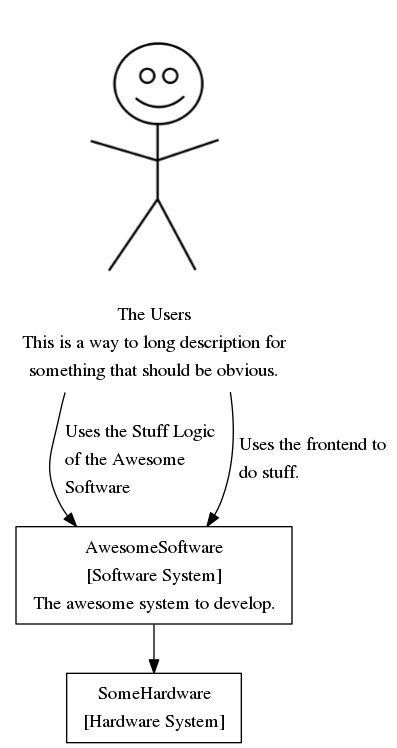
\includegraphics[width=1.0\paperwidth]{theworld.png}
	\end{textblock*}
\end{frame}

\begin{frame}
	\frametitle{The World and Containers}
	\begin{textblock*}{0cm}(-1.2cm,-2.0cm)
		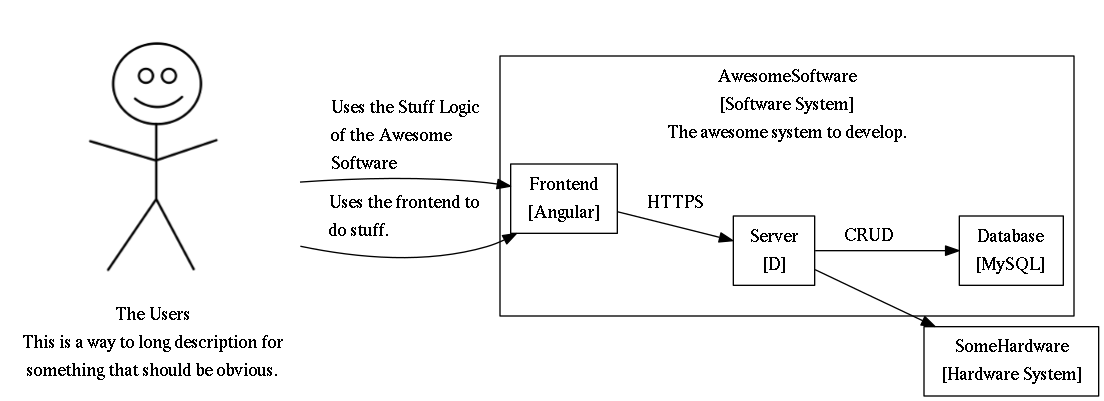
\includegraphics[width=1.0\paperwidth]{theworldandcontainer.png}
	\end{textblock*}
\end{frame}

%\begin{frame}
%	\frametitle{Actors, Containers and Components}
%	\begin{textblock*}{0cm}(-1.2cm,-2.0cm)
%		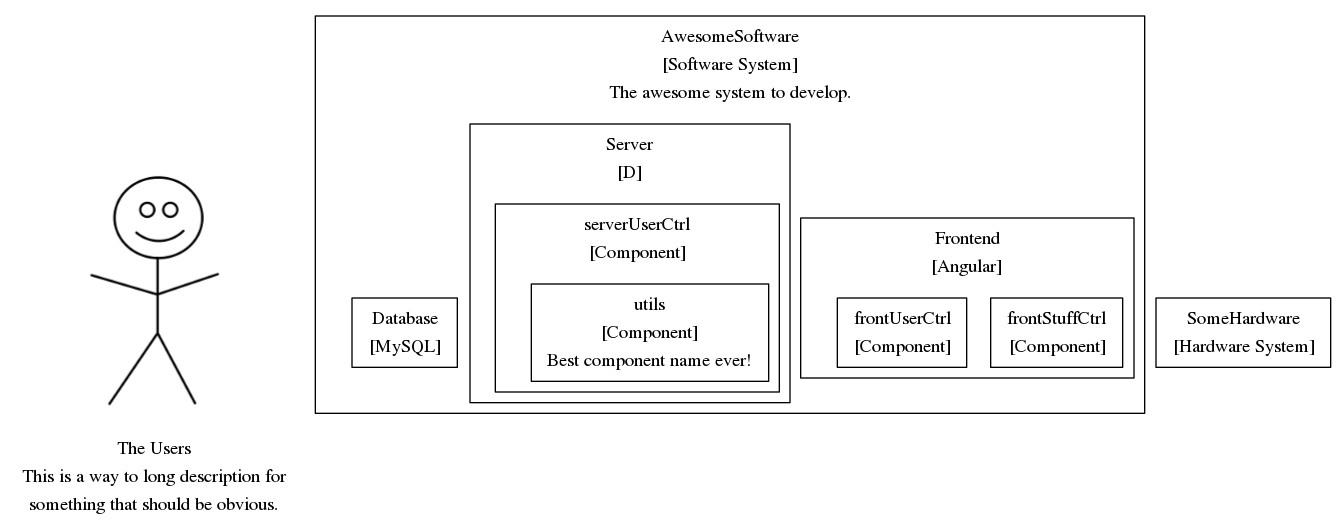
\includegraphics[width=1.0\paperwidth]{theworldcontainercomponents.png}
%	\end{textblock*}
%\end{frame}

\begin{frame}
	\frametitle{Awesome Software System}
	\begin{textblock*}{0cm}(-1.0cm,-4.0cm)
		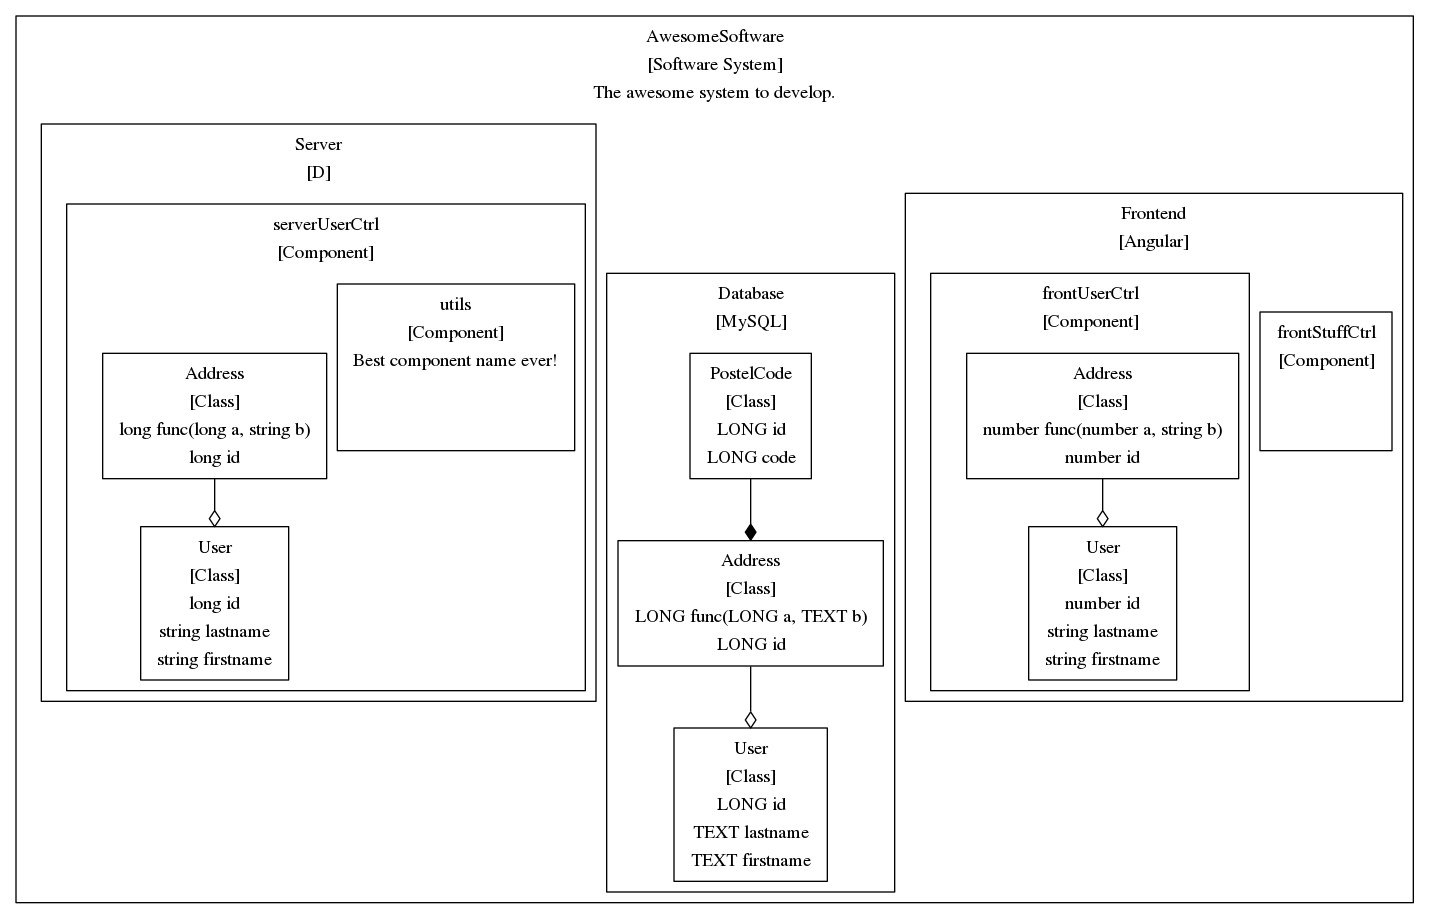
\includegraphics[width=1.0\paperwidth]{AwesomeSoftware.png}
	\end{textblock*}
\end{frame}

\begin{frame}
	\frametitle{Generating the Database CREATE TABLE Statements}
\begin{columns}[T]
\begin{column}{0.49\linewidth}
	\lstinputlisting[basicstyle=\scriptsize,language=SQL,caption={},
			numbers=none,xleftmargin=-0.5cm]
	{Sources/Address.sql}
	\vspace{12mm}
	\lstinputlisting[basicstyle=\scriptsize,language=SQL,caption={},numbers=none
		,xleftmargin=-0.5cm]
	{Sources/Address_User.sql}
\end{column}
\begin{column}{0.49\linewidth}
	\lstinputlisting[basicstyle=\scriptsize,language=SQL,caption={},numbers=none
		,xleftmargin=-0.4cm]
	{Sources/User.sql}
	\lstinputlisting[basicstyle=\scriptsize,language=SQL,caption={},numbers=none
			,xleftmargin=-0.4cm]
	{Sources/PostelCode.sql}
\end{column}
		
\end{columns}
\end{frame}

\begin{frame}
	\frametitle{What can we generate}
	\begin{itemize}
		\item Diagrams describing the project at different levels of detail
		\item Database schema
		\item phpmyadmin clones
		\item Database access code
		\item Data objects (D struct/class, Typescript interface/class, \(\dots\)
		\item Server skeletons
		\item Frontend skeletons
			\pause
		\item Graphviz mostly done, MySQL is getting there, Vibe.d and
			Angular2 next
	\end{itemize}
\end{frame}

\begin{frame}[plain]
\begin{textblock*}{0cm}(-1cm,-4.2cm)
	
\includegraphics[width=1.0\paperwidth]{picardpuppy.png}
	\todo{http://gryphon-shifter.deviantart.com/art/Captain-Picard-and-Puppies-458352865}
\end{textblock*}
\end{frame}

\begin{frame}
	\frametitle{The End}
	\begin{itemize}
		\item vibe.d \url{https://vibed.org}
		\item typescript \url{https://www.typescriptlang.org/}
		\item dstructtotypescript
			\url{https://github.com/burner/dstructtotypescript}
		\item C4 Architecture (Simon Brown) \url{http://www.codingthearchitecture.com}
		\item Structurizr \url{https://structurizr.com/}
		\item Degenerator \url{https://github.com/burner/Degenerator}
	\end{itemize}
\end{frame}

\end{document}
